\section{Калибровка электромагнитного калориметра}

\subsection{Псевдообратная матрица}

В линейном приближении зависимость энерговыделения в $i,j$-ой ячейке $E_{ij}$
от зарегистрированной амплитуды выражается как $E_{ij} = C_{ij} A_{ij}$, где
$C_{ij}$ -- калибровочный коэффициент. Тогда то свойство центральных
ячеек $I_c = ((2,3), (3,3))$, что ECAL практически полностью поглощает
всю энергию первичной частицы $E_{beam}$ в случае попадания частицы в них
можно записать следующим образом:
\begin{equation}
    E_{beam} = \sum\limits_{i,j}^{5,6} C_{ij} A_{ij},
    \label{eq:ecal-eSum}
\end{equation}
то есть, для герметичного калориметра, сумма энергий выделившихся во всех
ячейках должна быть равна номинальной энергии пучка для случая попадания
чавстицы в центральную часть (ячейки $(2,2)$ или $(2,3)$). Выражение
\eqref{eq:ecal-eSum} задаёт систему линейных уравнений.

Для идеального детектора можно было бы рассматривать $A_{ij}$ в смысле
средних значений для $N$ событий~$\bar{A}_{ij}=\mathop{\mathbb{E}}\limits_{n \in N}[A_{ij} + \delta A_{n,ij}] \simeq A_{ij}$, и тогда задача калибровки свелась
бы к решению простой СЛАУ. В реальности решения~\eqref{eq:ecal-eSum} для
каких-нибудь тридцати событий в общем
случае не существует, потому что для каждого события $n$
выражение~\eqref{eq:ecal-eSum} приобретает случайные добавки в каждой ячейке:
\begin{equation}
    E_{beam} + \delta E_n = \sum\limits_{i,j}^{5,6} \left( C_{ij} (A_{ij} + \delta A_{n,ij}) + \delta E_{n,ij} \right),
    \label{eq:ecal-eSum-deviating}
\end{equation}
где $\delta E_n,~\delta A_{n,ij}$ -- случайные значения отклонений энергии
частицы и зарегистрированной амплитуды, а $\delta E_{n,ij}$ -- физические флуктуации
в ячейке.

Тем не менее, в предположении, что для заданной средней координаты
падения частицы в среднем, энерговыделение в ячейке имеет нормальный
закон распределения $E_{ij} \sim \mathcal{N}(\bar{E}_{i,j},\sigma_{E,ij})$,
выражение \eqref{eq:ecal-eSum} задаёт \emph{переобусловленную} СЛАУ,
которую можно решить методом псевдообратной матрицы. Такая численная процедура
решает задачу минимизации среднего квадрата отклонения, и позволяет получить
приближённое решение~\eqref{eq:ecal-eSum}. Тем не менее, большое значение
для периферийных ячеек имеют флуктуации энерговыделения на
периферии ливня. Это приводит к большой ошибке в определении калибровочных
коэффициентов, если рассматривать только центральные ячейки для которых
выполняется условие герметичности.

Алгебраическую постановку задачи можно расширить, если рассмотреть
интеграл функции энерговыделения в объёме ячейки $v_{ij}$:
\begin{equation}
    E_{ij} =\int\limits_{v_{ij}} \frac{dE_{cnv} (r)}{d r} dv, \quad E_{beam} = \sum\limits_{ij}^{5,6} E_{i,j},
\end{equation}
где средняя объёмная дифференциальная плотность
энерговыделения $d E_{cnv}(r)/dr$ выражается через интегральную свёртку
проекции пучка $P$ на переднюю грань калориметра и функции объёмного
профиля ливня~$d E_{EM}(r)/dr$:
\begin{equation}
    E_{cnv}(r) = P * E_{EM}
        = \int\limits_{V} P(\rho_x,\rho_y) \frac{dE_{EM} (r -\rho)}{d \rho} d\rho.
    \label{eq:cnv-em-shower}
\end{equation}

Нужно заметить, что выражение \eqref{eq:cnv-em-shower} пренебрегает угловой
зависимостью импульсов частиц. В более общей постановке $E_{cnv}$
зависит от угла попадания частицы в калориметр, а $d E_{EM}/dr$ должна
учитывать анизотропию развития ливня в сэмплирующем калориметре.

Таблица значений $E_{ij}$ определяется относительно центральной
ячейки $i=0,j=0$. Таким образом для калориметра $5\times6$
$i$ изменяется в диапазоне от $-5$ до $5$ и $j$ от $-6$ до $6$.

\subsection{Координатная неоднородность}

Неоднородность отклика установки по отношению к точке попадания
инициирующей частицы в ECAL
иллюстрирует рисунок \ref{fig:ecal-cell-nonhomo}. Слева
изображена двумерная гистограмма заполненная координатным распределением
точки попадания частицы в локальных координатах, полученная экстраполяцией
на основе данных трекера. Резкий внешний круговой контур
соответствует проекции чувствительного элемента пучкового счётчика.
Локальные изменения плотности пятна соответствуют
конструктивным элементам ячейки калориметра в торцевой проекции изображённой
на рисунке справа -- по сравнению с центральной частью ячейки заметны
значительные (до $5~\text{ГэВ}$) флуктуации в оценке энергии ливня
при попадания частицы в армирующие стальные стержни
и на границах ячейки.
%или в отверстия через
%которые через ячейку проходят светопроводящие волокна.

%\begin{figure}
%    \centering
%    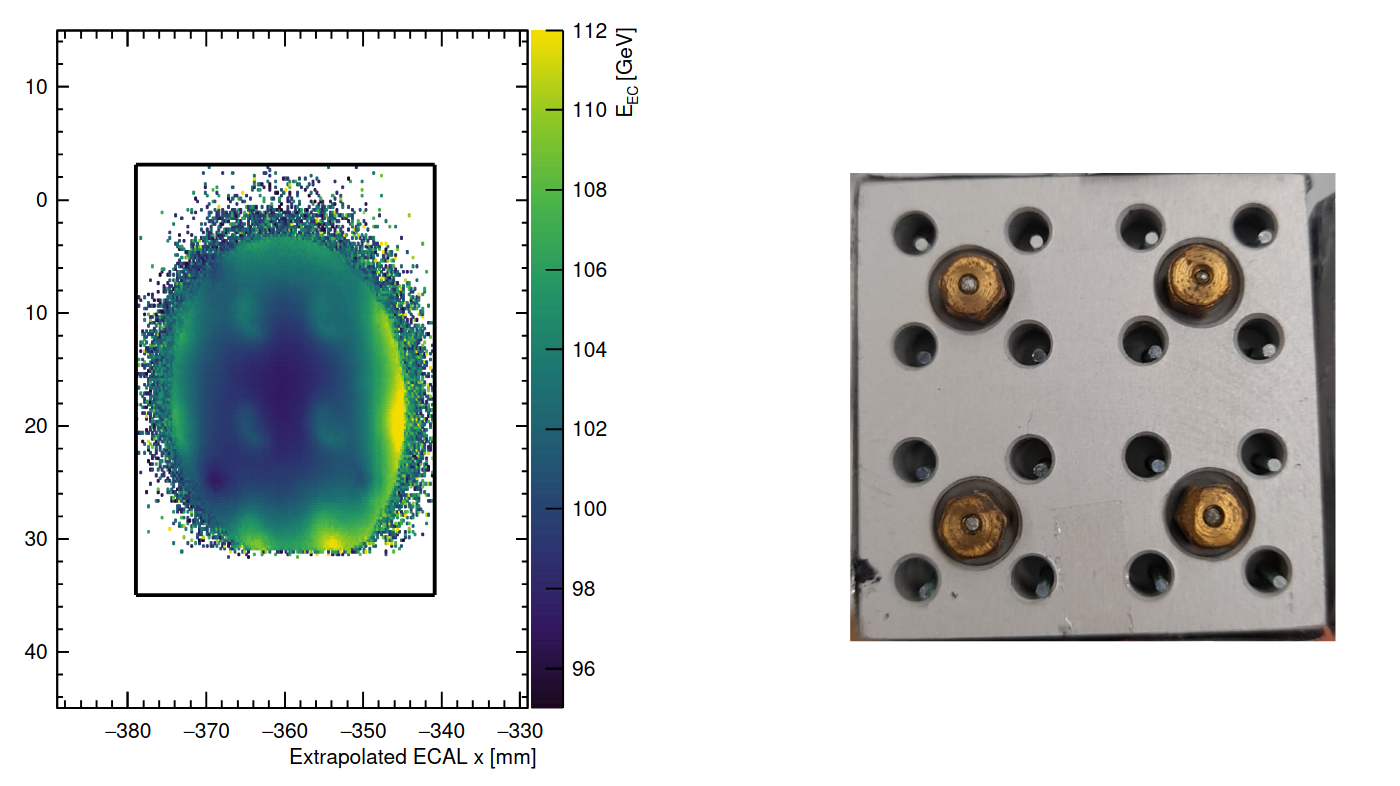
\includegraphics[width=0.95\linewidth]{images//illustrative/ECAL-cell-beamspot-nonhomo.png}
%    \caption{Распределение координат первичных частиц на фронтальной
%    грани калориметра ECAL и фотография торцевой части ячейки}
%    \label{fig:ecal-cell-nonhomo}
%\end{figure}

\begin{figure}
    \centering
    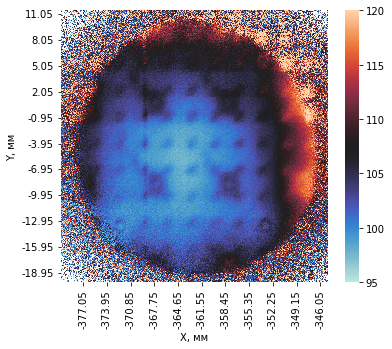
\includegraphics[width=0.45\linewidth]{images//illustrative/image.png}
    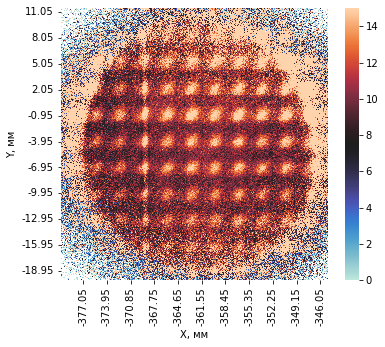
\includegraphics[width=0.45\linewidth]{images//illustrative/ecal-beam-error.png}
    \caption{Распределение среднего энерговыделения и
    абсолютной ошибки реконструкции энергии (ГэВ)}
    \label{fig:ecal-cell-nonhomo}
\end{figure}

Нестабильность поля отклоняющей магнитной системы способна вызывать
значительные горизонтальные колебания пучка. Рисунок~\ref{fig:counts-fluctuating}
иллюстрирует изменение числа зарегистрированных частиц из-за
кратковременного дрейфа координаты вызванного неполадками в питающей
системе отклоняющего магнита. На рисунке~\ref{fig:edep-fluctuations} приведена
скоррелированная зависимость изменения энерговыделения в центральной ячейке.

\begin{figure}
    \centering
    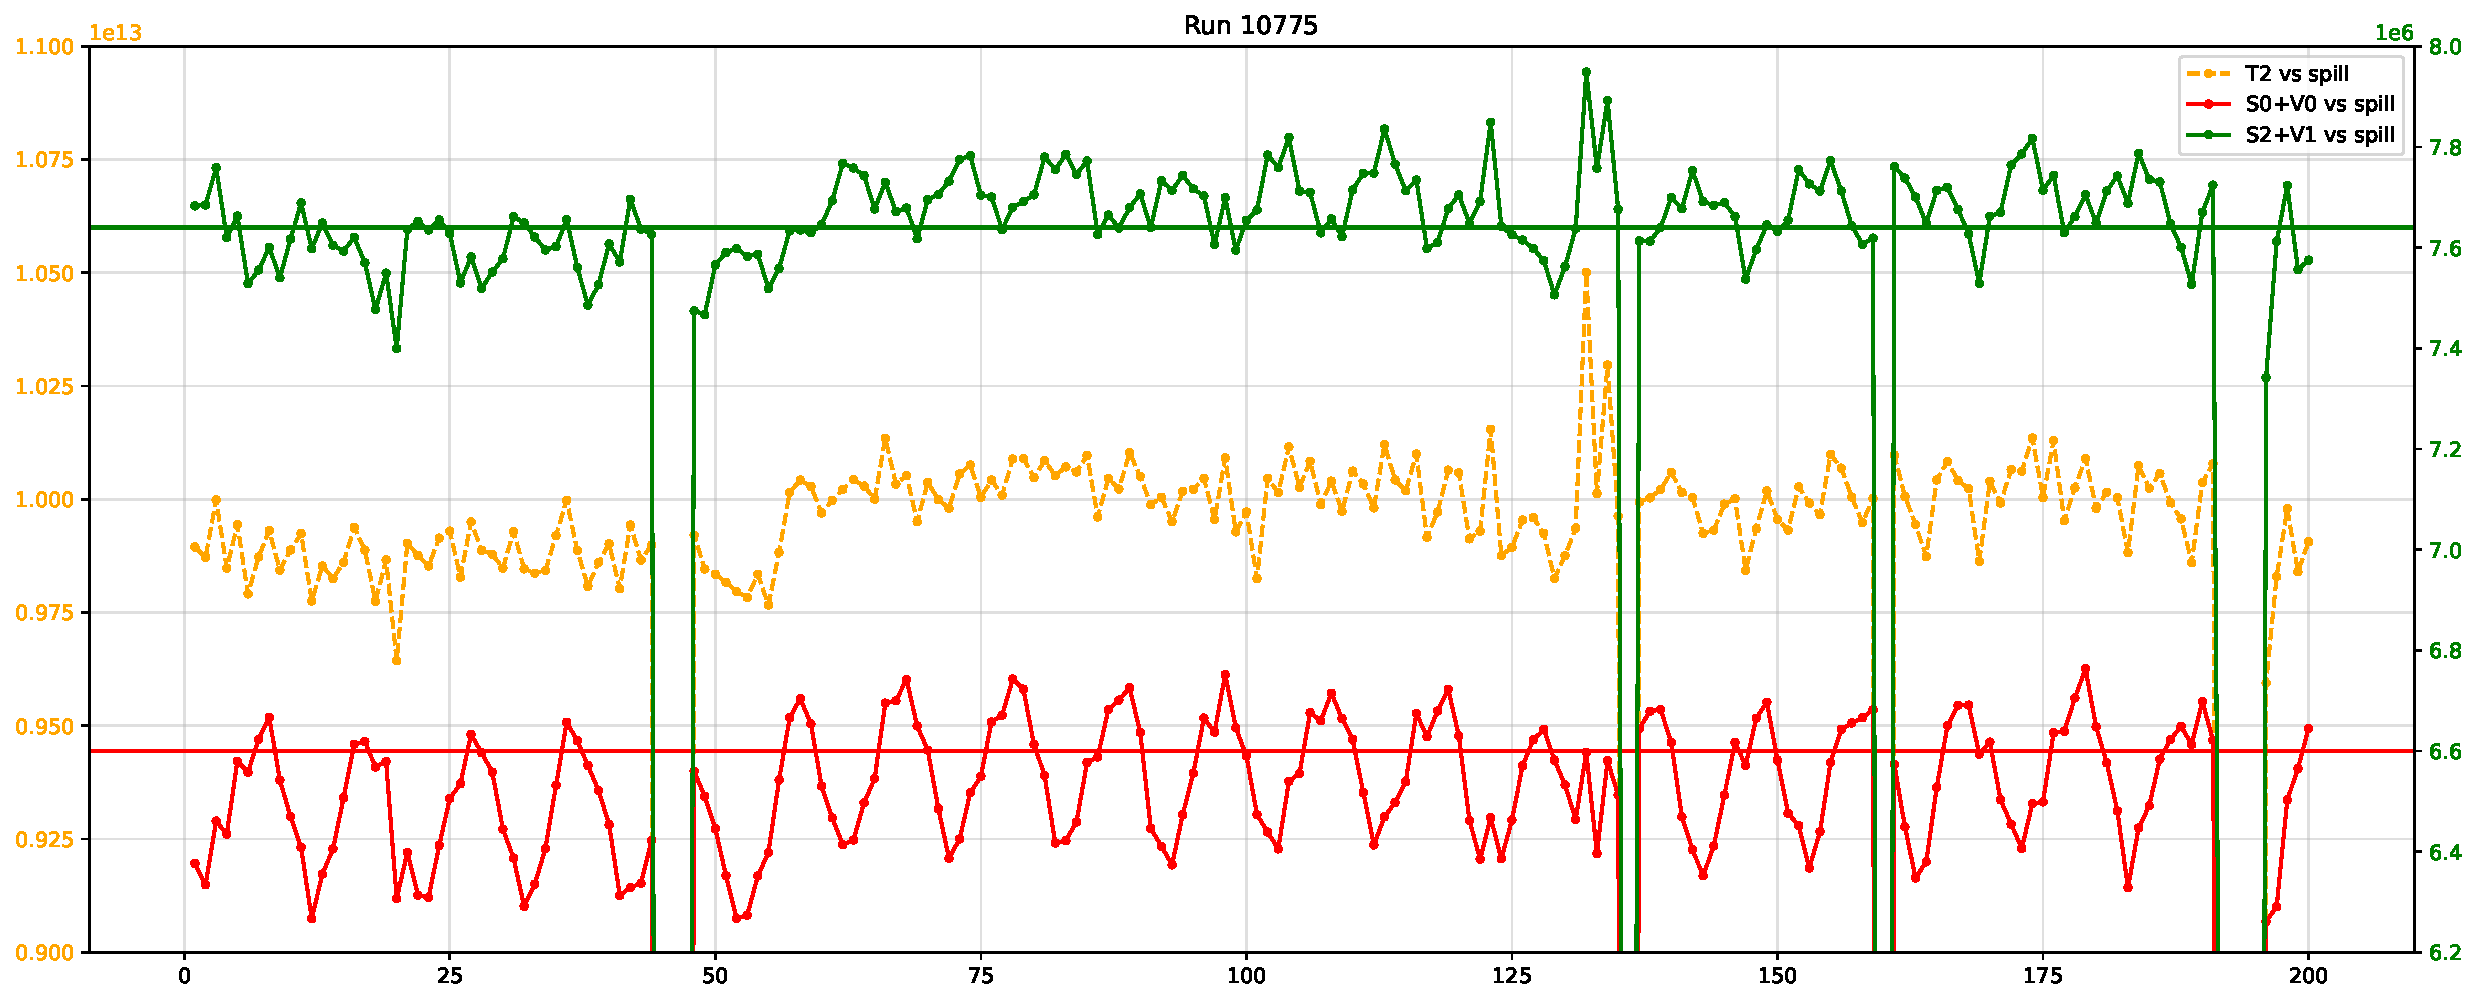
\includegraphics[width=0.95\linewidth]{images/illustrative/run-10775-t2-s0pv0-s2pv1.pdf}
    \caption{Развёртка числа частиц зарегистрированных на мишени (T2) и
    числа отсчётов пучковых счётчиков по номеру спилла}
    \label{fig:counts-fluctuating}
\end{figure}

\begin{figure}
    \centering
    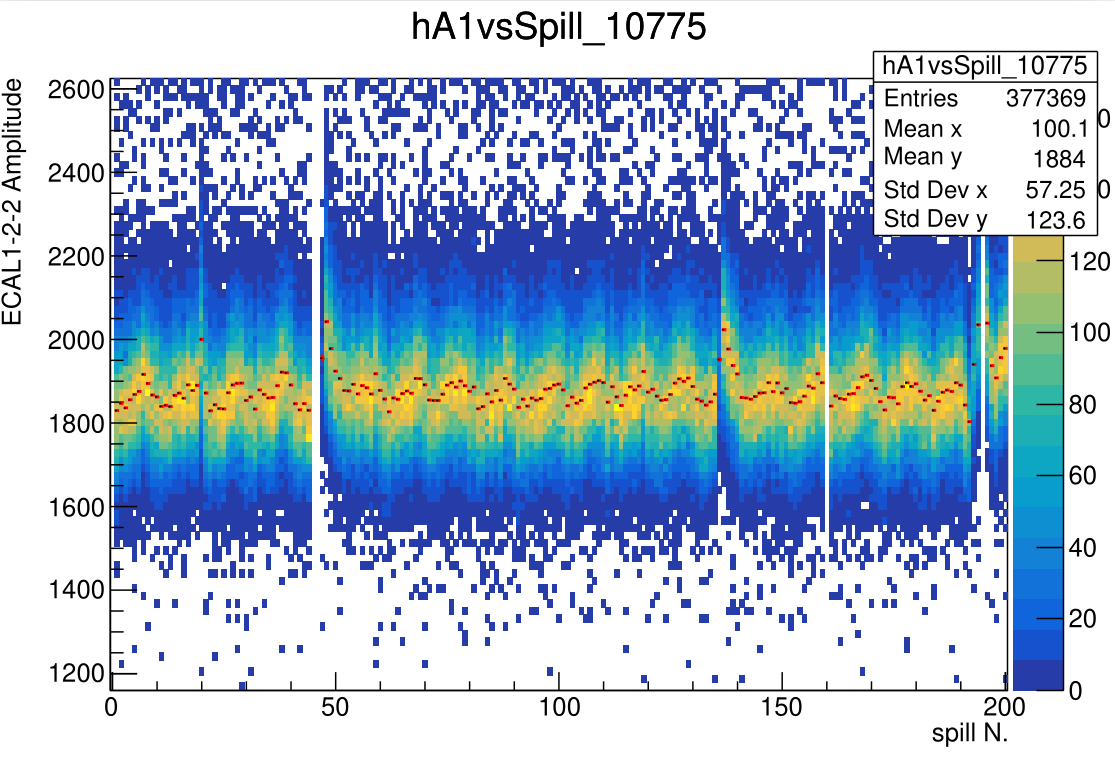
\includegraphics[width=1\linewidth]{images//illustrative/edep-fluctuations-run10775.png}
    \caption{Развёртка амплитудных показаний центральной ячейки ECAL}
    \label{fig:edep-fluctuations}
\end{figure}

Хотя данный случай носит исключительный характер (неполадки устранены),
он наглядно иллюстрирует необходимость привлечения информации о
треке частицы для оценок линейности калориметра, собственного
разрешения калориметра и т.д., поскольку ошибка энергетической
реконструкции вызванная неоднородной чувствительностью калориметра
может достигать нескольких процентов энерговыделения.

\subsection{Разрешение и линейность}

На рисунке~\ref{fig:ecal-linearity-test} изображены результаты
реконструкции энерговыделения для различных номинальных энергий
электронного пучка: $20~\text{ГэВ}$, $50~\text{ГэВ}$, $70~\text{ГэВ}$,
$80~\text{ГэВ}$, $100~\text{ГэВ}$.

\begin{figure}
    \centering
    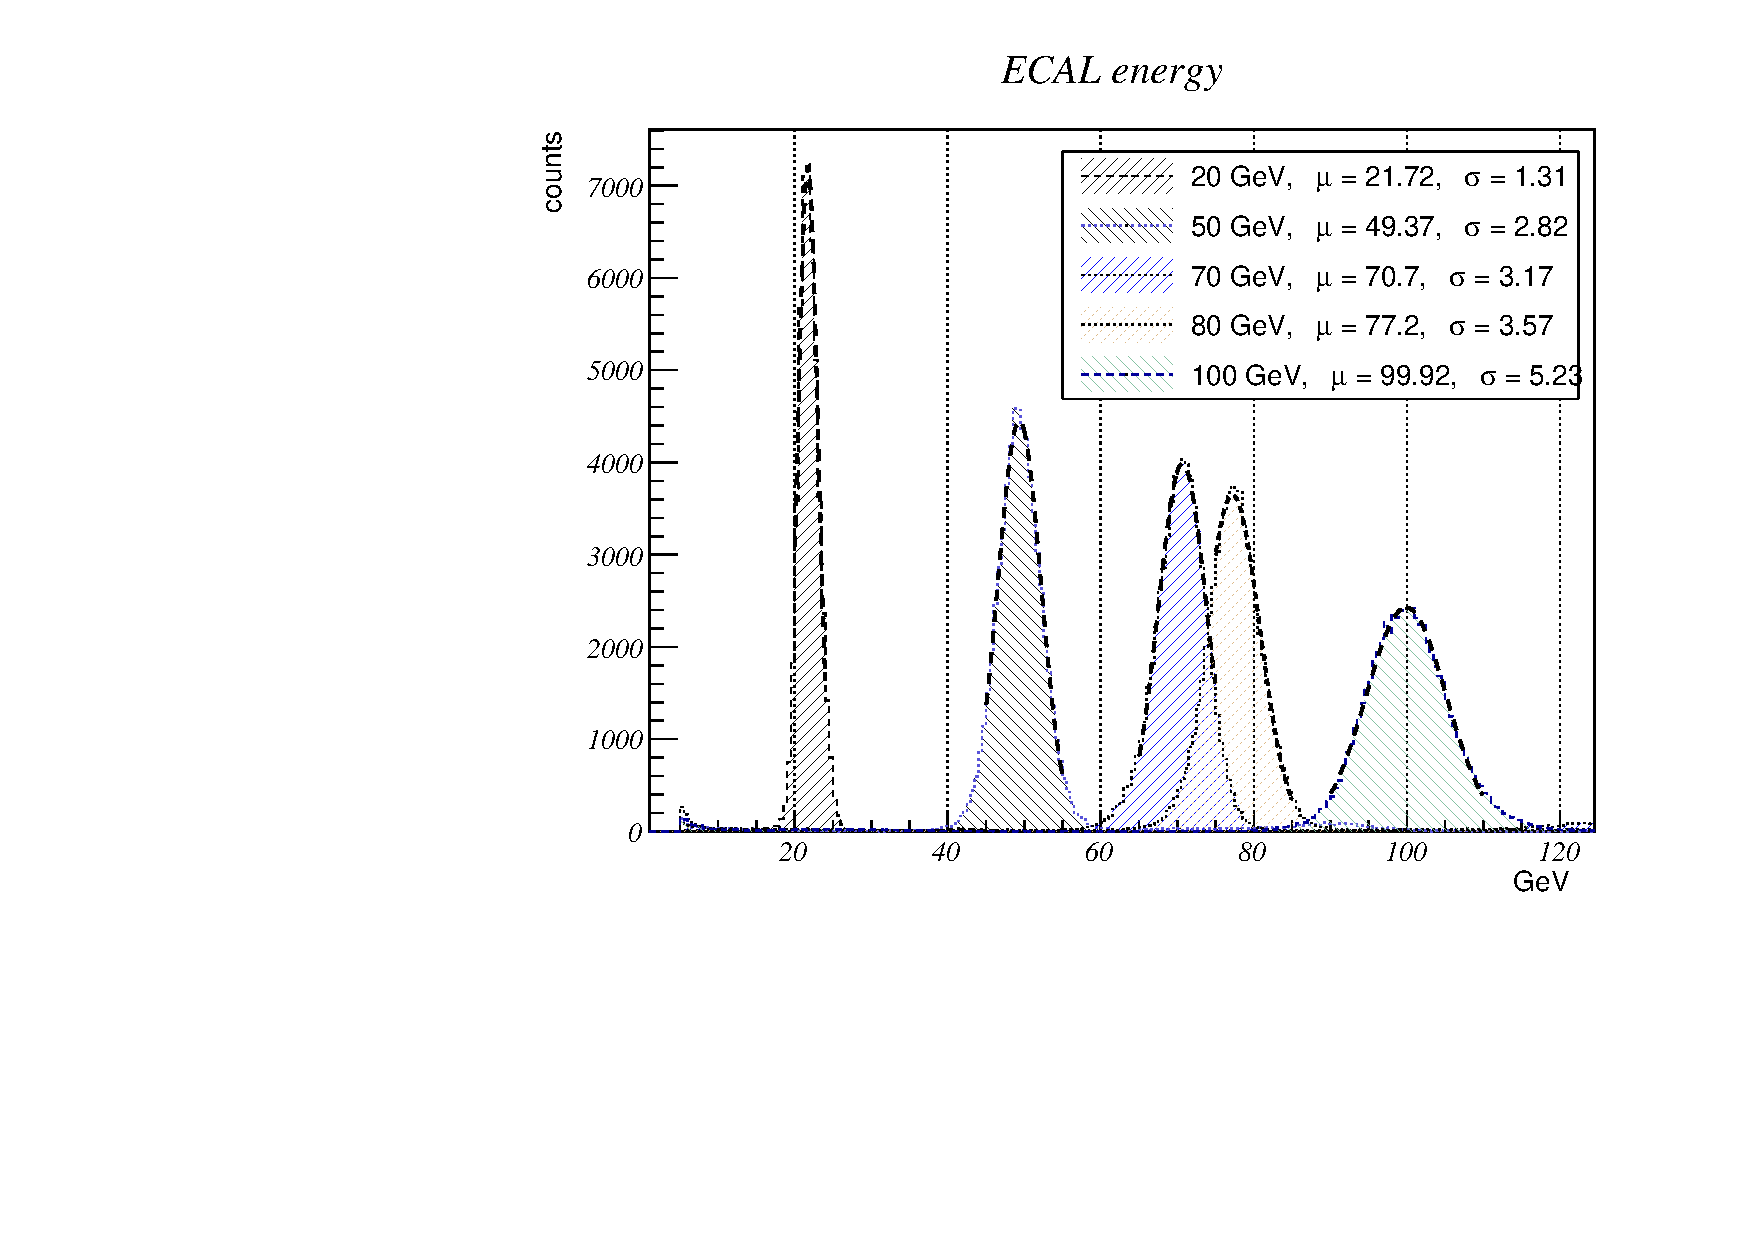
\includegraphics[width=0.75\linewidth]{images/lintest-2.pdf}
    \caption{Энергетический спектр в электромагнитном калориметре
    для различных энергий пучка}
    \label{fig:ecal-linearity-test}
\end{figure}
